\chapter{Введение в Концепции Программирования}\label{chapter:introduction_to_programming_concepts}

\epigraph{``Царской дороги в геометрии нет.''}{--- ответ Евклида Птолемею, \emph{Евклид} (около 300 лет до н. э.)}

\epigraph{``Следуй по дороге из жёлтого кирпича.''}{--- Удивительный волшебник из страны Оз, \emph{Лаймен Фрэнк Баум} (1856 - 1919)}

Программирование --- это указание компьютеру о том как он должен выполнять свою работу. В этой главе содержится простое, практическое введение в наиболее важные концепции программирования. Мы предполагаем что увы уже имели некоторый опыт работы с компьютерами. Мы используем интерактивный интерфейс Моцарт для постепенного введения в концепции программирования. Мы настоятельно рекомендуем вам пробовать выполнять приведённый в книге код на системе Моцарт.

В введении мы поверхностно рассматриваем концепции программирования. В последующих главах мы глубже рассматриваем эти концепции и добавляем множество других концепций и техник.

\section{Калькулятор}\label{section:Calculator}

Начнём с использования системы для выполнения вычислений. Запустим систему Моцарт напечатав:

\begin{lstlisting}
oz
\end{lstlisting}

или дважды кликнув мышью по иконке Моцарт. Будет открыто окно редактора с двумя областями. В верхней области напечатайте следующую строку: 

\begin{lstlisting}
{Browse 9999*9999}
\end{lstlisting}

Используйте мышь для выделения строки. Теперь перейдите в меню \verb|Oz| и выберите \verb|Feed Region|. Выделенный текст будет передан в систему. Система выполнит вычисление \lstinline!9999*9999! и отобразит результат, \lstinline!99980001!, в специальном окне под названием \emph{браузер (browser)}. Фигурные скобки \lstinline!{ ... }! используются для вызова процедуры или функции. \lstinline!Browse! --- это процедура с одним аргументом, и вызывается как \lstinline!{Browse X}!. Будет открыто окно браузера, если оно уже не открыто, и в нём будет отображено \lstinline!X!.

\section{Переменные}

При работе с калькулятором, нам может понадобиться запомнить старый результат для того, чтобы не печатать его ещё раз. Мы можем сделать это объявив \emph{переменную (variable)}:

\begin{lstlisting}
declare
V=9999*9999
\end{lstlisting}

Так мы объявили \lstinline!V! и привязали его к \lstinline!99980001!. Мы можем использовать эту переменную в последующих вычислениях:

\begin{lstlisting}
{Browse V*V}
\end{lstlisting}

Будет дан ответ \lstinline!9996000599960001!.

Переменные --- это всего лишь ярлыки для значений. То есть, они не могут быть присвоены более одного раза. Но, вы \emph{можете} определить другую переменную с тем же именем, что и предыдущая переменная. Это означает что старая переменная уже станет недоступной. Но предыдущие вычисления, использовавшие старую переменную, не изменятся. А происходит это потому, что за словом ``переменная'' скрываются две концепции:

\begin{itemize}
\item{\emph{Идентификатор}. Это то, что вы печатаете. Переменные начинаются с заглавной буквы и могут быть продолжены любыми буквами или цифрами. Например, заглавная буква ``\lstinline!V!'' может быть идентификатором переменной.}

\item{\emph{Сохраняемое значение}. Это то, что используется системой для вычислений. Часть системной памяти, которую мы называем сохранённой.}
\end{itemize}

Оператор \lstinline!declare! создаёт новое сохранённое значение и делает так, что идентификатор переменной начинает ссылаться на это значение. Старые вычисления, использующие аналогичный идентификатор \lstinline!V!, не будут изменяться, поскольку идентификатор относится к другой переменной.

\section{Функции}\label{section:Functions}

А теперь выполним более сложный расчёт. Предположим что нам нужно вычислить функцию факториал $n!$, которая определяется как $1 \times 2 \times \cdot \cdot \cdot \times (n-1) \times n$. У нас получаются количество перестановок из $n$ элементов, то есть, количество разнообразных способов размещения этих элементов в строку. Факториал $10$:

\begin{lstlisting}
{Browse 1*2*3*4*5*6*7*8*9*10}
\end{lstlisting}

Будет отображено $3628800$. А если мы захотим вычислить факториал $100$? Мы были бы непротив если бы система выполнила за нас эту утомительную работу по печати целых чисел от $1$ до $100$. Мы сделаем даже больше: мы объясним системе как вычислить факториал для любых $n$. Мы сделаем это определив функцию:

\begin{lstlisting}
declare
fun {Fact N}
   if N==0 then 1 else N*{Fact N-1} end
end
\end{lstlisting}

Ключевое слово \lstinline|declare| обозначает что мы хотим определить нечто новое. Ключевое слово \lstinline|fun| обозначает начало новой функции. Функция называется \lstinline|Fact| и имеет один аргумент \lstinline|N|. Аргумент является локальной переменной, то есть, известен только внутри тела функции. Каждый раз мы вызываем функцию с новой объявленной переменной.

\subsection{Рекурсия}

Тело функции --- это инструкция с выражением \lstinline|if|. При вызове функции выражение \lstinline|if| выполняет следующие шаги:

\begin{itemize}

  \item{Первым делом выполняется проверка на равенство $N$ нулю с помощью выполнения теста \lstinline|N==0|.}

\item{Если тест завершился успешно, то вычисляется выражение после \lstinline|then|. В данном случае просто возвращается число \lstinline|1|. Происходит это потому что факториал $0$ равен $1$.}


\item{Если тест провалился, то вычисляется выражение после \lstinline|else|. Таким образом если $N$ не равен $0$, то выполняется выражение \lstinline|N*{Fact N-1}|. Это выражение использует \lstinline|Fact|, функцию, которую мы уже определили! Это называется \emph{рекурсией (recursion)}. Это абсолютно нормально и нет причин для тревоги. \lstinline|Fact| рекурсивен поскольку факториал $N$ --- это просто $N$ умноженный на факториал $N-1$. \lstinline|Fact| использует следующее математическое определение факториала:

  $$
  \begin{array}{l}
    0! = 1 \\
    n! = n \times (n-1)! \text{ если } n > 0
  \end{array}
$$

а это рекурсия.}
\end{itemize}

Теперь мы можем попробовать запустить функцию:

\begin{lstlisting}
  {Browse {Fact 10}}
\end{lstlisting}


В результате будет отображено $3628800$. Можно быть уверенным, что \lstinline|Fact| выполняет верные вычисления. А теперь попробуем ввести более крупный ввод:

\begin{lstlisting}
  {Browse {Fact 100}}
  \end{lstlisting}

Будет отображено \emph{огромное} число:

$$
  \begin{array}{rrrrrrrr}
    933 & 26215 & 44394 & 41526 & 81699 & 23885 & 62667 & 00490 \\
    71596 & 82643 & 81621 & 46859 & 29638 & 95217 & 59999 & 32299 \\
    15608 & 94146 & 39761 & 56518 & 28625 & 36979 & 20827 & 22375 \\
    82511 & 85210 & 91686 & 40000 & 00000 & 00000 & 00000 & 00000
  \end{array}
$$


Это пример арифметики с независимой точностью, иногда называемой ``бесконечной точностью'', хотя она и не является бесконечной. Точность ограничивается количеством памяти в вашей системе. Типичные персональные компьютеры низкого ценового диапазона с 64 MB памяти может обрабатывать сотни из тысяч цифр. Скептически настроенный читатель может спросить: действительно ли это огромное число является факториалом 100? Как мы можем это проверить? Выполнение ручного вычисления займёт много времени и возможно результат будет неверным. Позже мы увидим как можно проверить корректность работы системы.

\subsection{Комбинации}

Напишем функцию, вычисляющую число комбинаций $r$ элементов из $n$ элементов. Это равносильно числу подмножеств размером $r$, которые можно собрать из набора размером $n$. В математическом виде записывается как $\begin{pmatrix} n \\ r \end{pmatrix}$ и произносится ``$r$ выбранные из $n$''. И может быть определено с помощью использования факториала:

$$
\begin{pmatrix} n \\ r \end{pmatrix} = \frac{n!}{r! (n - r)!}
$$

что дословно можно переписать в следующую функцию:

\begin{lstlisting}
declare
fun {Comb N R}
   {Fact N} div ({Fact R}*{Fact N-R})
end
\end{lstlisting}

Например, \lstinline|{Comb 10 3}| даёт $120$, являющееся числом способов с помощью которых можно выбрать $3$ элемента из $10$. Способ с помощью которого написан \lstinline|Comb| не самый эффективный, но, скорее всего, самый простой.

\subsection{Функциональные абстракции}

Функция \lstinline|Comb| вызывает \lstinline|Fact| три раза. Всегда возможно использовать существующие функции для облегчения определения новых функций. Этот принцип называется \emph{функциональной абстракцией ({\selectlanguage{english}functional abstraction})}, поскольку использует функции для постройки абстракций. Таким образом, большие программы похожи на лук, то есть, слой на слое из функций, вызывающих функции.

\section{Списки}

Теперь мы можем вычислять целые числа с помощью функций. Но сами по себе целые числа не столь интересны. Предположим что нам нужно вычислять лишь некоторые целые числа. Например, мы можем захотеть вычислить треугольник Паскаля:

$$
\begin{array}{ccccccccccc}
  & & & & &1& & & & & \\
  & & & &1& &1& & & & \\
  & & &1& &2& &1& & & \\
  & &1& &3& &3& &1& & \\
  &1& &4& &6& &4& &1& \\
 \cdot&\cdot&\cdot&\cdot&\cdot&\cdot&\cdot&\cdot&\cdot&\cdot&\cdot \\
  \end{array}
$$

\newcommand\consgraph[3]{
  % #1 - X, #2 - Y, #3 - надпись на car-е
  \draw (#1, #2) -- (#1, #2 - 0.5);
  \draw [->] (#1, #2 - 0.5) -- (#1 - 0.5, #2 - 1.5) node [below] {#3};
  \draw [->] (#1, #2 - 0.5) -- (#1 + 0.5, #2 - 1.5);
  \node [below left] at (#1, #2 - 0.9) {\tiny{1}};
  \node [below right] at (#1, #2 - 0.9) {\tiny{2}};
}




Этот треугольник назван в честь учёного и мистика Блеза Паскаля. Он начинается с $1$ в первой строке. Каждый элемент представляет сумму двух других вышестоящих элементов: правого и левого. (Если соседних элементов нет, например на грани, то в качестве недостающего элемента берут ноль.) Мы хотели бы определить одну функцию, которая формирует $n$-ую строку за один раз. $N$-ая строка содержит $n$ целых чисел. Мы можем реализовать такую функцию с помощью \emph{списков} целых чисел.



Список --- это всего лишь последовательность элементов, окружённая скобками справа и слева, например \lstinline|[5 6 7 8]|. По историческим причинам, пустой список пишется как \lstinline|nil| (а не \lstinline|[]|). Списки могут отображаться как числа:

\begin{lstlisting}
  {Browse [5 6 7 8]}
\end{lstlisting}

Запись вида \lstinline|[5 6 7 8]| --- это просто сокращение. На самом деле список --- это \emph{цепь из ссылок}, где каждая ссылка содержит две вещи: один элемент списка и указатель на остальную часть цепи. Списки всегда создаются из \emph{одного элемента}, начинаются с \lstinline|nil| и к нему добавляются один за другим ссылки. Новая ссылка пишется как \lstinline!H|T!, где \lstinline|H| --- это новый элемент и \lstinline|T| --- старая часть цепи. Построим список. Мы начнём с \lstinline|Z=nil|. Мы добавим первую ссылку \lstinline!Y=7|Z!, а затем вторую ссылку \lstinline!X=6|Y!. Теперь \lstinline|X| ссылается на список из двух ссылок, а сам список может быть написан как \lstinline|[6 7]|.

Ссылка \lstinline!H|T! часто называется как \emph{cons}, это термин, который пришёл к нам из Лиспа\footnote{Большинство списковой терминологии возникло вместе с появлением языка Лисп в конце 1950 годов и с тех пор так и прижилось \cite{120}. Использование вертикальной разделительной черты пришло из Prolog, языка логического программирования, изобретённого в начале 1970 годов \cite{40, 182}. В Лиспе cons записывается как \lstinline|(H . T)|, что называется \emph{точечной парой}.}. Также мы называем ссылку \emph{парой списка}. Создание новых ссылок называется \emph{консингом (consing)}. Если \lstinline|T| --- это список, то консинг \lstinline|H| и \lstinline|T| создаёт новый список \lstinline!H|T!:



\begin{lstlisting}
declare
H=5
T=[6 7 8]
{Browse H|T}
\end{lstlisting}

Список \lstinline!H|T! может быть записан как \lstinline|[5 6 7 8]|. Здесь \emph{голова (head)} $5$ и \emph{хвост (tail)} \lstinline|[6 7 8]|. Cons \lstinline!H|T! можно разобрать и вернуться к голове и хвосту:

\begin{lstlisting}
declare
L=[5 6 7 8]
{Browse L.1}
{Browse L.2}
\end{lstlisting}

\begin{figure}[h]
  \begin{tikzpicture}
    \node [align=left] at (0, 10) {\lstinline|L = [5 6 7 8]                                  L.1 = 5|                                 \\
      \lstinline|L =                                            L.2 = [6 7 8]| \\
      \lstinline|                                               L.2 =|};
    \consgraph{-4}{10}{$5$}
    \consgraph{-3.5}{8.5}{$6$}
    \consgraph{-3}{7}{$7$}
    \consgraph{-2.5}{5.5}{$8$}
    \node [below] at (-2, 4) {\lstinline|nil|};
    \consgraph{4}{9.5}{$6$}
    \consgraph{4.5}{8}{$7$}
    \consgraph{5}{6.5}{$8$}
    \node [below] at (5.5, 5) {\lstinline|nil|};
    \node at (1, 8) {$\Longrightarrow$};
  \end{tikzpicture}
  \caption{Конструкция списка \lstinline|[5 6 7 8]|}
  \label{figure:list_construction}
\end{figure}

Здесь применяется оператор точка ``\lstinline|.|'', служит для выбора первого или второго аргумента из пары списка. Выполнение \lstinline|L.1| возвращает голову \lstinline|L|, целочисленное \lstinline|5|. Выполнение \lstinline|L.2| возвращает хвост \lstinline|L|, список \lstinline|[6 7 8]|. Рис.~\ref{figure:list_construction} изображает строение списка: \lstinline|L| --- это цепь, в которой каждое звено обладает одним списковым элементом и \lstinline|nil| обозначает конец. Выполнение \lstinline|L.1| возвращает первый элемент, а выполнение \lstinline|L.2| возвращает остальную часть цепи.

\subsection{Сравнение с шаблоном}\label{Pattern_Matching}

Мы можем сократить нашу работу и получить части списка воспользовавшись инструкцией \lstinline|case|, за один шаг получающей голову и хвост:

\begin{lstlisting}
declare
L=[5 6 7 8]
case L of H|T then {Browse H} {Browse T} end
\end{lstlisting}

Возвращаются \lstinline|5| и \lstinline|[6 7 8]|, также, как и в примере выше. Инструкция \lstinline|case| определяет две локальные переменные, \lstinline|H| и \lstinline|T|, и привязывает их к голове и хвосту списка \lstinline|L|. Мы говорим что инструкция \lstinline|case| выполняет \emph{сравнение с шаблоном (pattern matching)}, поскольку она выполняет разложение \lstinline|L| в соответствии с ``шаблоном'' \lstinline!H|T!. Локальные переменные определённые в \lstinline|case| --- подобны переменным, определённым с помощью \lstinline|declare|, с тем исключением что переменные существуют только в теле оператора \lstinline|case|, то есть, между \lstinline|then| и \lstinline|end|.

\section{Функции для работы над списками}\label{section_functions_over_lists}

\begin{figure}[h]
\begin{tikzpicture}
  \node (one) at (6, 5) {1};
  \node (twoone) [below left= 0.5cm of one] {1};
  \node (twotwo) [below right=0.5cm of one] {1};
  \node (threeone) [below left=0.5cm of twoone] {1};
  \node (threetwo) [below right=0.5cm of twoone] {2};
  \node (threethree) [below right=0.5cm of twotwo] {1};
  \node (element_2) [below left=0.5cm of threeone] {1};
  \node (element_3) [below left=0.5cm of threetwo] {3};
  \node (element_4) [below right=0.5cm of threetwo] {3};
  \node (element_5) [below right=0.5cm of threethree] {1};
  \node (element_11) [below left=0.5cm of element_2] {1};
  \node (element_12) [below right=0.5cm of element_2] {4};
  \node (element_13) [below right=0.5cm of element_3] {6};
  \node (element_14) [below right=0.5cm of element_4] {4};
  \node (element_15) [below right=0.5cm of element_5] {1};
  \node (element_1) [above left=0.5cm of element_11] {(0)};
  \node (element_6) [above right=0.5cm of element_15] {(0)};
  \draw [->] (element_1) -- (element_11);
  \draw [->] (element_2) -- (element_11);
  \draw [->] (element_2) -- (element_12);
  \draw [->] (element_3) -- (element_12);
  \draw [->] (element_3) -- (element_13);
  \draw [->] (element_4) -- (element_13);
  \draw [->] (element_4) -- (element_14);
  \draw [->] (element_5) -- (element_14);
  \draw [->] (element_5) -- (element_15);
  \draw [->] (element_6) -- (element_15);
  \node [above=0.125cm of element_11] {$+$};
  \node [above=0.125cm of element_12] {$+$};
  \node [above=0.125cm of element_13] {$+$};
  \node [above=0.125cm of element_14] {$+$};
  \node [above=0.125cm of element_15] {$+$};
%  
  
  
  \node (label4) [right=0.5cm of element_6] {\emph{4-я строка}};
  \node (label3) [above=0.2cm of label4] {\emph{3-я строка}};
  \node (label2) [above=0.2cm of label3] {\emph{2-я строка}};
  \node (label1) [above=0.2cm of label2] {\emph{1-я строка}};
  \node (label5) [below=0.2cm of label4] {\emph{5-я строка}};
\end{tikzpicture}
\caption{Вычисление пятой строки треугольника Паскаля}
\label{figure:Fifth_row}
\end{figure}

Теперь, когда мы можем производить вычисления над списками, определим функцию, \lstinline|{Pascal N}|, предназначенную для вычисления $n$-ой строки треугольника Паскаля. Для начала разберём вычисление вручную. Рис.~\ref{figure:Fifth_row} иллюстрирует вычисление пятой строки, основанное на четвёртой строке. Рассмотрим механизм вычисления в случае когда каждая строка представляет список из целых чисел. Вычисление текущей строки мы начинаем с предыдущей строки. Мы сдвигаем её налево на одну позицию и сдвигаем направо на одну позицию. Дальше мы складываем вместе две сдвинутые строки. Например возьмём четвёртую строку:

\begin{lstlisting}
  [1 3 3 1]
\end{lstlisting}

Мы сдвинули эту строку влево и вправо и сложили получившиеся строки вместе:

\begin{lstlisting}
  [1 3 3 1 0]
+ [0 1 3 3 1]
\end{lstlisting}

Заметьте, что сдвиг влево добавляет ноль справа, а сдвиг налево добавляет ноль слева. Выполнение сложения даёт следующий результат:

\begin{lstlisting}
  [1 4 6 4 1]
\end{lstlisting}

что является пятой строкой.

\subsection{Главная функция}\label{subsection:The_main_function}

Теперь, когда мы поняли как решать проблему, мы можем написать функцию, выполняющую те же операции. Вот она:

\begin{lstlisting}
declare Pascal AddList ShiftLeft ShiftRight
fun {Pascal N}
   if N==1 then [1]
   else
      {AddList {ShiftLeft {Pascal N-1}}
       {ShiftRight {Pascal N-1}}}
   end
end
\end{lstlisting}

В дополнение к определению \lstinline|Pascal| мы определили переменные для трёх дополнительных функций, которые ещё нужно определить.

\subsection{Дополнительные функции}\label{subsection:The_auxiliary_functions}

Проблема решена не до конца. Мы дополнительно определили ещё три функции: \lstinline|ShiftLeft|, сдвигающую влево на одну позицию, \lstinline|ShiftRight|, сдвигающую вправо на одну позицию и \lstinline|AddList|, складывающую два списка. Вот \lstinline|ShiftLeft| и \lstinline|ShiftRight|:

\begin{lstlisting}
fun {ShiftLeft L}
   case L of H|T then
      H|{ShiftLeft T}
   else [0] end
end

fun {ShiftRight L} 0|L end
\end{lstlisting}

\lstinline|ShiftRight| всего лишь добавляет ноль слева. \lstinline|ShiftLeft| проходит через \lstinline|L| по одному элементу за раз и строит вывод также в один элемент за единицу времени. Мы добавили \lstinline|else| в инструкцию \lstinline|case|. Аналогично \lstinline|else| в \lstinline|if|: исполняется при несовпадении с шаблоном \lstinline|case|. Таким образом, если \lstinline|L| окажется пустым, то на выходе будет \lstinline|[0]|, то есть, список с единственным нулём внутри.

Вот \lstinline|AddList|:

\begin{lstlisting}
fun {AddList L1 L2}
   case L1 of H1|T1 then
      case L2 of H2|T2 then
         H1+H2|{AddList T1 T2}
      end
   else nil end
end
\end{lstlisting}

Это самая сложная функция из всех виденных на данный момент. Она использует две \lstinline|case| инструкции, одна в другой, поскольку нам нужно разобрать два списка, \lstinline|L1| и \lstinline|L2|. Теперь, когда у нас есть полное определение \lstinline|Pascal|, мы можем вычислить любую строку из треугольника Паскаля. Например, вызов \lstinline|{Pascal 20}| вернёт 20-ю строку:

\begin{lstlisting}
  [1 19 171 969 3876 11628 27132 50388 75582 92378 92378 75582 50388 27132 11628 3876 969 171 19 1]
\end{lstlisting}

Это правильный ответ? Как это можно доказать? Он выглядит правильным: он симметричен (если написать его справа налево, то мы получим тот же список) и первый и второй аргументы равны $1$ и $19$, что тоже правильно. Взглянув на рис.~\ref{figure:Fifth_row}, можно увидеть что второй элемент $n$-ой строки всегда $n-1$ (он всегда на единицу больше предыдущей строки и для первой строки начинается с ноля). В следующем разделе мы узнаем как надо выяснять корректность.

\subsection{Разработка программ методом свер\-ху\--вниз}

Просуммируем технику, применённую для написания \lstinline|Pascal|:

\begin{itemize}
\item{Первый шаг --- это выяснение выполнения вычислений и ручное воспроизведение вычислений.}

\item{Второй шаг --- это написание главной функции, решающей нашу задачу, \emph{предполагая} что некоторые вспомогательные функции (в нашем примере, \lstinline|ShiftLeft|, \lstinline|ShiftRight| и \lstinline|AddList|) уже известны.}

\item{Третий шаг --- это завершение решения через написание вспомогательный функций.}
\end{itemize}

Техника, по которой вначале пишут главную функцию, а потом заполняют пробелы известна как разработка программного обеспечения \emph{сверху-вниз}. Эта техника --- одна из наиболее известных подходов, но она всего лишь одна часть целой истории.

\section{Корректность}\label{section:Correctness}

Программа корректна тогда, когда она выполняет то, что мы от неё хотим. Как мы можем доказать что программа корректна? Обычно невозможно повторить программные вычисления вручную. Нам нужен другой способ. Один из простых способов, который мы уже применяли заключается в том, чтобы проверить программу на уже заранее известных данных. Это повышает доверие к программе. Но на этот способ нельзя полностью положиться. Для того, чтобы в целом доказать корректность, надо произвести рассуждения о программе. Это означает три вещи:

\begin{itemize}
\item{Нам нужна математическая модель операций языка программирования, объясняющая выполняемые действия. Эта модель называется \emph{семантикой} языка.}

\item{Нам нужно определить то, что мы хотим получить от программы. Обычно это обозначает математическое определение входных данных, требуемых программой, и выходные данные, которые она должна вычислить. Это называется \emph{спецификацией} программы.}

\item{Мы применяем математические техники для построения рассуждений о программе основываясь на семантике. Нам нужно продемонстрировать что программа удовлетворяет спецификации.}
\end{itemize}

Программа, для которой доказана её корректность, может возвращать некорректные результаты, если система, на которой она запущена, реализована некорректно. Как нам убедиться что система удовлетворяет семантике? Здесь нужно выполнить проверку: это означает проверку компилятора, исполняющей системы, операционной системы и даже аппаратного обеспечения! Это важная тема, но освещение этой темы лежит за пределом этой книги. В этой книге мы доверяемся разработчикам Моцарта, компаниям, выпускающим программное обеспечение и производителям аппаратного обеспечения.\footnote{Некоторые скажут что это звучит глупо. Перефразируя Томаса Джефферсона, они скажут что цена корректности --- это вечная бдительность.}



\subsection{Математическая индукция}

Математическая индукция --- это одна из очень полезных техник. Она заключается в двух шагах. Вначале нам нужно показать что программа корректна для простых случаев. Далее нам нужно показать, что если программа корректна для простого случая, то она будет корректной и для следующего случая. Исходя из этих двух шагов, математическая индукция позволяет нам сделать вывод о том, что программа будет всегда корректной. Эта техника может быть применена для целочисленных значений и списков:

\begin{itemize}
\item{Для целочисленных значений базовым случаем является $0$ или $1$, а для данного целого числа $n$ следующим случаем будет $n+1$.}

\item{Для списков базовым случаем будет \lstinline|nil| (пустой список) или список с одним или несколькими элементами, и для данного \lstinline|T| списка следующим случаем будет \lstinline!H|T! (без условий для \lstinline|H|).}
\end{itemize}

Рассмотрим как применяется индукция для функции факториала:

\begin{itemize}

\item{\lstinline|{Fact 0}| возвращает правильный ответ, а именно, \lstinline|1|.}

\item{Предположим, что \lstinline|{Fact N-1}| корректен. Тогда рассмотрим вызов \lstinline|{Fact N}|. Мы увидим что инструкция \lstinline|if| выполняет случай \lstinline|else|, и вычисляет \lstinline|N*{Fact N-1}|. По условию, \lstinline|{Fact N-1}| возвращает правильный ответ. Таким образом, предположив что умножение тоже возвращает правильный результат, \lstinline|{Fact N}| также возвращает правильный ответ.}
\end{itemize}

Это рассуждение использует математическое определение факториала, а именно: $n! = n \times (n - 1)!$ если $n > 0$, и $0! = 1$. Дальше в этой книге мы увидим более сложные техники рассуждений. Но, базовый подход всегда остаётся тем же самым: начинаем с семантики языка и спецификации задачи и применяем математические рассуждения для доказательства того, что программа корректно реализует спецификацию.

\section{Сложность}\label{section:complexity}

Функция \lstinline|Pascal|, уже определённая нами выше, работает \emph{очень медленно} если мы попытаемся вычислить строки с большим номером. Вычисление строки $20$ займёт по времени около двух или одной секунд. Вычисление $30$-й строки уже займёт значительное количество минут. Если вы запустите это вычисление, то приготовьтесь к длительному ожиданию. В чём причина столь долгой работы? Давайте ещё раз взглянем на функцию \lstinline|Pascal|:

\begin{lstlisting}
fun {Pascal N}
   if N==1 then [1]
   else
      {AddList {ShiftLeft {Pascal N-1}}
       {ShiftRight {Pascal N-1}}}
   end
end
\end{lstlisting}


Вызов \lstinline|{Pascal N}| приведёт к двукратному вызову \lstinline|{Pascal N-1}|. Таким образом, вызов \lstinline|{Pascal 30}| приведёт к двукратному вызову \lstinline|{Pascal 29}|, что в свою очередь приведёт к четырёхкратному вызову \lstinline|{Pascal 28}|, к восьмикратному \lstinline|{Pascal 27}| и так далее, удваивая каждый следующий ряд. В результате у нас получается $2^{29}$ вызовов \lstinline|{Pascal 1}|, а это примерно равно полмиллиарду вызовов. Нет ничего удивительного в том, что \lstinline|{Pascal 30}| настолько медлителен. Можем ли мы ускорить его? Да, есть один простой способ: достаточно вызывать \lstinline|{Pascal N-1}| один раз, а не дважды. Поскольку второй вызов возвращает тот же результат что и первый вызов, то нам будет достаточно запомнить первый вызов. Мы можем запомнить его воспользовавшись локальной переменной. Вот новая функция \lstinline|FastPascal|, использующая локальную переменную:

\begin{lstlisting}
fun {FastPascal N}
   if N==1 then [1]
   else L in
      L={FastPascal N-1}
      {AddList {ShiftLeft L} {ShiftRight L}}
   end
end
\end{lstlisting}


Мы определили локальную переменную \lstinline|L| добавив ``\lstinline|L in|'' в \lstinline|else|. Всё равно что использование \lstinline|declare|, с тем исключением что переменная будет существовать между \lstinline|else| и \lstinline|end|. Мы привязали \lstinline|L| к результату \lstinline|{FastPascal N-1}|. Теперь мы можем использовать \lstinline|L| везде, где только захотим. Насколько быстр \lstinline|FastPascal|? Попробуйте вычислить $30$-ю строку. В случае с \lstinline|Pascal| потребуются минуты, но \lstinline|FastPascal| отрабатывает практически мгновенно. Урок, который мы можем извлечь из этого примера, говорит о том, что использование хорошего алгоритма более важно чем наличие самого лучшего компилятора или самой быстрой машины.

\subsection{Время выполнение (run-time) гарантирует исполнение программы в течение определённого времени}

Как показывает пример выше, очень важно иметь сведения о времени выполнения программы. Знание, касающееся времени, затраченного на выполнение программы менее важно нежели знание того, что время не будет расти взрывообразно с ростом входных данных. Время, затраченное на исполнение программы можно рассматривать как или функцию от входных данных, или константу и называющуюся \emph{временн\'{о}й сложностью (time complexity)}. Эта функция зависит от изменения размеров входных данных. Мы предполагаем что эта функция зависит от того как используется программа. Например, входной размер \lstinline|{Pascal N}| будет простым целочисленным \lstinline|N| (а не, например, количеством памяти, требуемой для хранения \lstinline|N|).

Временн\'{а}я сложность \lstinline|{Pascal N}| пропорциональна $2^n$. Это экспоненциальная функция от $n$, растущая очень быстро при увеличении $n$. Какова временная сложность \lstinline|{FastPascal N}|? Есть $n$ рекурсивных вызовов, и каждый вызов создаёт список со средним размером $n/2$. Таким образом временная сложность пропорциональна $n^2$. Эта полиномиальная функция от $n$, растущая гораздо меньше чем экспоненциальная функция. Программы с экспоненциальной временной сложностью непрактичны за исключением очень малых входных данных. И наоборот, программы с низкой полиномиальной временной сложностью --- практичны.

\section{Ленивое вычисление}\label{section:lazy_evaluation}

Функции, которые мы до сих пор писали, выполняют вычисления сразу же после вызова. Такое поведение называется \emph{энергичным вычислением (eager evaluation)}. Другой способ вычисления функций называется \emph{ленивым вычислением (lazy evaluation)}.\footnote{Иногда называется как \emph{вычисление управляемое данными (data-driven)} и \emph{вычисление по-требованию (demand-driven)} соответственно.} В ленивом вычислении выполнение программы начинается только тогда, когда нужен результат. Вот простой пример ленивой функции, вычисляющей список целых чисел:

\begin{lstlisting}
fun lazy {Ints N}
   N|{Ints N+1}
end
\end{lstlisting}


Вызов \lstinline|{Ints 0}| вычисляет бесконечный список \lstinline!0|1|2|3|4|5|...! . Выглядит как бесконечный цикл, но это не так. Аннотация \lstinline|lazy| указывает что функция будет вычисляться только тогда, когда будет нужен результат. В этом одно из достоинств ленивого вычисления: мы можем вычислять потенциально бесконечные структуры данных без всяких условий, ограничивающих цикл. Например:

\begin{lstlisting}
L={Ints 0}
{Browse L}
\end{lstlisting}


Будет отображено следующее, то есть, почти ничего:

\begin{lstlisting}
L<Future>
\end{lstlisting}

(Браузер отобразит значения, не влияющие на их вычисление.) Аннотация ``\lstinline|Future|'' означает что \lstinline|L| обладает ленивой функцией, присоединённой к нему. Если потребуется значение \lstinline|L|, то эта функция будет автоматически вызвана. Таким образом, для того, чтобы получить результаты, мы должны выполнить что-то, для чего требуется список. Например:

\begin{lstlisting}
  {Browse L.1}
\end{lstlisting}

Будет отображён первый элемент, а именно \lstinline|0|. Мы можем вычислить список так, как будто он уже существует:

\begin{lstlisting}
  case L of A|B|C|_ then {Browse A+B+C} end
\end{lstlisting}

Результатом будет вычисление только первых трёх элементов \lstinline|L| и ничего более. Что будет отображено?

\subsection{Ленивое вычисление треугольника Паскаля}

Сделаем что нибудь полезное с помощью ленивого вычисления. Было бы неплохо написать функцию, позволяющую вычислять столько строк треугольника Паскаля, сколько нам нужно, но, мы не знаем сколько строк нам нужно вычислить. Нам нужна возможность наблюдать ряды и самим решать когда их количество будет нас удовлетворять. Вот ленивая функция, которая генерирует бесконечный список строк:

\begin{lstlisting}
 fun lazy {PascalList Row}
   Row|{PascalList
        {AddList {ShiftLeft Row}
         {ShiftRight Row}}}
 end
\end{lstlisting}



Вызов функции и просмотр получившегося результата ничего нам не даст:

\begin{lstlisting}
declare
L={PascalList [1]}
{Browse L}
\end{lstlisting}

(Аргумент \lstinline|[1]| --- это первая строка треугольника.) Для того, чтобы получить больше результатов, нужно уведомить об этом систему:

\begin{lstlisting}
{Browse L.1}
{Browse L.2.1}
\end{lstlisting}

Будут отображены первая и вторая строки.

Вместо написания ленивой функции, мы могли бы написать функцию, получающую \lstinline|N|, число требуемых строк, и прямо вычисляющую эти строки, начиная с начальной строки:



\begin{lstlisting}
fun {PascalList2 N Row}
   if N==1 then [Row]
   else
      Row|{PascalList2 N-1
           {AddList {ShiftLeft Row}
            {ShiftRight Row}}}
   end
end
\end{lstlisting}


Мы можем отобразить $10$ строк с помощью вызова \lstinline|{Browse {PascalList2 10 [1]}}|. А вдруг позже нам понадобится $11$ строк? Нам придётся вызвать \lstinline|PascalList2| ещё раз, на этот раз с аргументом \lstinline|11|. Вся наша предыдущая работа по вычислению $10$ строк будет напрасной. Ленивая версия позволяет избежать необходимости в выполнении всей работы заново. Она всегда готова продолжить работу с того места, где произошла пауза.

\section{Высокоуровневое программирование}\label{section:higher-order_programming}

Мы написали эффективную функцию, \lstinline|FastPascal|, позволяющую вычислять строки треугольника Паскаля. Теперь было бы неплохо поэкспериментировать с различными вариациями треугольника Паскаля. Например, вместо сложения чисел для получения строки, мы могли бы вычитать их или применять к ним \lstinline|exclusive-or| (для вычисления чётности или нечётности) или какие-нибудь другие операции. Один из возможных способов --- это написать отдельную версию \lstinline|FastPascal|, реализующую какой-либо один вариант. Но подобный подход быстро становится утомительным. Можем ли мы вместо создания различных вариантов использовать какой-либо \emph{один} вариант? Это возможно. Назовём эту реализацию \lstinline|GenericPascal|. Всякий раз, когда мы вызываем её, мы будем передавать ей какую-либо изменяющуюся функцию (сложение, выяснение чётности и т.д.) в виде аргумента. Возможность передачи функций как аргументов известна как \emph{высокоуровневое программирование}.

Вот определение \lstinline|GenericPascal|. Она принимает ещё один аргумент, \lstinline|Op|, хранящий функцию, которая вычисляет каждое число:



\begin{lstlisting}
fun {GenericPascal Op N}
   if N==1 then [1]
   else L in
      L={GenericPascal Op N-1}
      {OpList Op {ShiftLeft L} {ShiftRight L}}
   end
end
\end{lstlisting}


\lstinline|AddList| заменён на \lstinline|OpList|. Дополнительный аргумент \lstinline|Op| передаётся в \lstinline|OpList|. \lstinline|ShiftLeft| и \lstinline|ShiftRight| не надо ничего знать об \lstinline|Op|, поэтому мы продолжаем использовать старые версии. Определение \lstinline|OpList|:

\begin{lstlisting}
fun {OpList Op L1 L2}
   case L1 of H1|T1 then
      case L2 of H2|T2 then
         {Op H1 H2}|{OpList Op T1 T2}
      end
   else nil end
end
\end{lstlisting}


Вместо сложения \lstinline|H1+H2| эта версия выполняет \lstinline|{Op H1 H2}|.

\subsection{Разновидности треугольника Паскаля}

Определим некоторые функции для того, чтобы испытать \lstinline|GenericPascal|. Для получения исходного треугольника Паскаля мы можем определить функцию сложения:

\begin{lstlisting}
fun {Add X Y} X+Y end
\end{lstlisting}

\VerbatimFootnotes
Теперь мы можем запустить \lstinline|{GenericPascal Add 5}|.\footnote{Мы могли бы вызвать \verb|{Browse {GenericPascal Number.|$'$\verb|+|$'$\verb| 5}}|, поскольку операция сложения  $'$\lstinline|+|$'$ --- это часть модуля \lstinline|Number|. Но в этой главе модули не упоминаются.} В результате мы получим всё ту же пятую строку. С помощью \lstinline|GenericPascal| мы можем определить \lstinline|FastPascal|:

\begin{lstlisting}
fun {FastPascal N} {GenericPascal Add N} end
\end{lstlisting}

Определим другую функцию:

\begin{lstlisting}
fun {Xor X Y} if X==Y then 0 else 1 end end
\end{lstlisting}

Эта функция реализует операцию \emph{исключающее ИЛИ}, определяемую так:

\begin{center}
\begin{tabular}{ccc}
\lstinline|X| & \lstinline|Y| & \lstinline|{Xor X Y}| \\
0 & 0 & 0 \\
0 & 1 & 1 \\
1 & 0 & 1 \\
1 & 1 & 0 \\
\end{tabular}
\end{center}

Исключающее ИЛИ позволяет вычислить \emph{чётность} каждого числа в треугольнике Паскаля, то есть, является ли число чётным или нечётным. Сами числа не вычисляются. Вызов \lstinline|{GenericPascal Xor N}| даст такой результат:

\begin{tikzpicture}
  \node (11) {1};

  \node (21) [below left = 0.5cm of 11] {1};
  \node (22) [below right = 0.5cm of 11] {1};

  \node (31) [below left = 0.5cm of 21] {1};
  \node (32) [below right = 0.5cm of 21] {0};
  \node (33) [below right = 0.5cm of 22] {1};

  \node (41) [below left = 0.5cm of 31] {1};
  \node (42) [below right = 0.5cm of 31] {1};
  \node (43) [below right = 0.5cm of 32] {1};
  \node (44) [below right = 0.5cm of 33] {1};

  \node (51) [below left = 0.5cm of 41] {1};
  \node (52) [below right = 0.5cm of 41] {0};
  \node (53) [below right = 0.5cm of 42] {0};
  \node (54) [below right = 0.5cm of 43] {0};
  \node (55) [below right = 0.5cm of 44] {1};

  \node (61) [below left = 0.5cm of 51] {1};
  \node (62) [below right = 0.5cm of 51] {1};
  \node (63) [below right = 0.5cm of 52] {0};
  \node (64) [below right = 0.5cm of 53] {0};
  \node (65) [below right = 0.5cm of 54] {1};
  \node (66) [below right = 0.5cm of 55] {1};

  \node (71) [below left = 0.5cm of 61] {1};
  \node (72) [below right = 0.5cm of 61] {0};
  \node (73) [below right = 0.5cm of 62] {1};
  \node (74) [below right = 0.5cm of 63] {0};
  \node (75) [below right = 0.5cm of 64] {1};
  \node (76) [below right = 0.5cm of 65] {0};
  \node (77) [below right = 0.5cm of 66] {1};

  \node (81) [below left = 0.5cm of 71] {$\cdot$};
  \node (82) [below right = 0.5cm of 71] {$\cdot$};
  \node (83) [below right = 0.5cm of 72] {$\cdot$};
  \node (84) [below right = 0.5cm of 73] {$\cdot$};
  \node (85) [below right = 0.5cm of 74] {$\cdot$};
  \node (86) [below right = 0.5cm of 75] {$\cdot$};
  \node (87) [below right = 0.5cm of 76] {$\cdot$};
  \node (88) [below right = 0.5cm of 77] {$\cdot$};
\end{tikzpicture}

Некоторые другие функции даны в упражнениях.

\section{Параллелизм}

Было бы неплохо если бы программа могла выполнять несколько действий и каждое действие могло выполняться обособленно. Это называется \emph{параллелизмом (concurrency)}. Между выполняемыми операциями не должно быть никаких взаимодействий, только если программист не решит что они должны обмениваться между собой информацией. Это отображение работы реального мира вне системы. Неплохо бы повторить это внутри системы.

Мы вводим параллелизм через создание нитей. \emph{Нить (thread)} --- это простое исполнение таких программ, как функции, которые мы видели ранее. Разница в том, что программа может содержать в себе более одной нити. Нити создаются с помощью инструкции \lstinline|thread|. Помните насколько медленной была исходная функция \lstinline|Pascal|? Мы могли вызывать \lstinline|Pascal| внутри его собственной нити. Это означает что \lstinline|Pascal| не будет выполнять никаких других вычислений. Если \lstinline|Pascal| будет выполнять много вычислений, то время ожидания может затянуться. А всё потому, что нити разделяют между собой один компьютер. Но, ни одна нить не будет останавливаться. Пример:

\begin{lstlisting}
thread P in
   P={Pascal 30}
   {Browse P}
end
{Browse 99*99}
\end{lstlisting}

Так мы создали новую нить. Внутри этой новой нити мы вызвали \lstinline|{Pascal 30}| и затем вызвали \lstinline|Browse| для отображения результата. Новая нить будет работать долгое время. Но это не остановит систему и она немедленно отобразит результат вычисления \lstinline|99*99|.

\section{Поток данных}

\begin{figure}
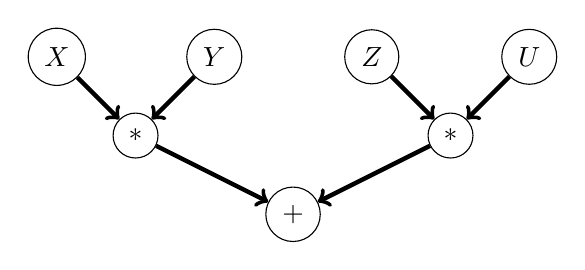
\begin{tikzpicture}
  \node [draw, circle] (X_node) at (1, 3) {$X$};
  \node [draw, circle] (Y_node) at (3, 3) {$Y$};
  \node [draw, circle] (Z_node) at (5, 3) {$Z$};
  \node [draw, circle] (U_node) at (7, 3) {$U$};
  
  \node [draw, circle] (First_mul) at (2, 2) {$*$};
  \node [draw, circle] (Second_mul) at (6, 2) {$*$};

  \node [draw, circle] (Addition_node) at (4, 1) {$+$};
  \draw [ultra thick, ->] (X_node) -- (First_mul);
  \draw [ultra thick, ->] (Y_node) -- (First_mul);

  \draw [ultra thick, ->] (Z_node) -- (Second_mul);
  \draw [ultra thick, ->] (U_node) -- (Second_mul);

  \draw [ultra thick, ->] (First_mul) -- (Addition_node);
  \draw [ultra thick, ->] (Second_mul) -- (Addition_node);
\end{tikzpicture}
\caption{Простой пример исполнения потока данных}
\label{figure:Dataflow_execution_simple_example}
\end{figure}
Что произойдёт если операция будет пытаться использовать переменную, которая ещё не была привязана? С чисто эстетической точки зрения было бы неплохо если бы операция просто дождалась привязки переменной. Возможно какая-нибудь другая нить привязала бы переменную, и после этого операция могла бы продолжиться. Это цивилизованное поведение известно под названием \emph{поток данных (dataflow)}. Рис.~\ref{figure:Dataflow_execution_simple_example} демонстрирует простой пример: два умножения ждут пока их аргументы будут привязаны и сложение ждёт пока не будут завершены операции умножения. Позже мы увидим что существует множество хороших причин по которым крайне желателен поток данных. А теперь, посмотрим как работает вместе поток данных и параллелизм. Возьмём такой пример:

\begin{lstlisting}
declare X in
thread {Delay 10000} X=99 end
{Browse start} {Browse X*X}
\end{lstlisting}

Умножение \lstinline|X*X| будет ждать до тех пор, пока не будет привязано значение \lstinline|X|. Первый \lstinline|Browse| незамедлительно отобразит \lstinline|start|. Второй \lstinline|Browse| будет ожидать окончания перемножения, и поэтому ничего не отобразит. Вызов \lstinline|{Delay 10000}| создаст паузу на $10000$ миллисекунд (то есть, на $10$ секунд). \lstinline|X| будет привязан только по прошествии паузы. Когда \lstinline|X| будет привязан, тогда будет продолжена операция умножения и сработает второе \lstinline|Browse|, отображающее $9801$. Две операции \lstinline|X=99| и \lstinline|X*X| могут выполняться в любом порядке с паузами любой продолжительности; поток данных всегда будет возвращать один результат. Замедление вычисления результата может вызвать только эффект паузы. Например:

\begin{lstlisting}
declare X in
thread {Browse start} {Browse X*X} end
{Delay 10000} X=99
\end{lstlisting}

Поведение такое же что и в предыдущем примере: браузер отобразит $9801$ после $10$ секунд. Это иллюстрация двух удобных особенностей потока данных. Первое, вычисления работают корректно вне зависимости от того как они разбиты между нитями. Второе, вычисления терпеливы: они не порождают сигналы об ошибках, а просто ждут.

Добавление нитей и задержек в программу может коренным образом изменить внешний вид программы. Но, пока вызываются одни и те же операции с одними и теми же аргументами, то результаты программы будут неизменными. Это ключевая особенность параллелизма потока данных. Вот почему параллелизм потока данных позволяет использовать большинство преимуществ параллелизма попутно избежав сложностей, обычно ассоциируемых с ним.

\section{Состояние}

Как сделать так, чтобы функция могла знать что происходило с ней в прошлом? Это означает что функция должна обладать некоторой внутренней памятью, которая бы помогала ей выполнять свою работу. Память нужна функциям, которые могут изменять своё поведение и знать своё прошлое. Эта разновидность памяти называется \emph{явным состоянием (explicit state)}. Как и параллелизм, модели явного состояния --- это важные аспекты отображающие работу настоящего мира. И нам нужно смоделировать их в нашей системе. В дальнейшем, по мере чтения, вы увидите более глубокие причины для явного состояния. Ну а теперь, рассмотрим работу состояния.

Например, нам может понадобиться знать как часто была использована функция \lstinline|FastPascal|. Каким способом \lstinline|FastPascal| может запомнить количество предыдущих вызовов? Мы реализуем это через добавление явного состояния.

\subsection{Ячейка памяти}

Есть несколько способов определения явного состояния. Простейший способ --- это определение единственной \emph{ячейки памяти (memory cell)}. Это некая разновидность ящика в который вы можете помещать произвольное содержимое. Многие языки программирования называют этот ящик ``переменной''. Мы называем её ``ячейкой'' для того, чтобы избежать путаницы с ранее использованными переменными, которые скорее подобны математическим переменным, то есть, простые обозначения некоторых значений. Для ячеек существует три функции: \lstinline|NewCell| создаёт новую ячейку, \lstinline|:=| (присваивание) вставляет новое значение в ячейку и \lstinline|@| (доступ) получает текущее значение, сохранённое в ячейке. Доступ и присваивание также называются как чтение и запись. Например:

\begin{lstlisting}
declare
C={NewCell 0}
C:=@C+1
{Browse @C}
\end{lstlisting}

Тут создаётся ячейка \lstinline|C| с инициализирующим содержимым $0$, содержимое увеличивается на единицу и отображается содержимое ячейки \lstinline|C|.

\subsection{Добавление памяти к FastPascal}

Благодаря ячейки памяти мы можем добавить \lstinline|FastPascal| возможность подсчитывать количество вызовов. Для начала мы создадим ячейку за пределами \lstinline|FastPascal|. Затем внутри \lstinline|FastPascal| мы добавим единицу к содержимому ячейки. Результат будет таким:

\begin{lstlisting}
declare
C={NewCell 0}
fun {FastPascal N}
   C:=@C+1
   {GenericPascal Add N}
end
\end{lstlisting}

(Ради сокращения это определение использует \lstinline|GenericPascal|.)

\section{Объекты}\label{section:objects}

Функции с внутренней памятью, обычно, называются \emph{объектами (objects)}. Таким образом определённая в предыдущем разделе расширенная версия \lstinline|FastPascal| является объектом. Оказывается что объекты --- это очень полезные звери. Дадим другой пример. Мы определим объект-счётчик. Счётчик обладает ячейкой, в которой хранит текущий счёт. У счётчика есть две операции, \lstinline|Bump| и \lstinline|Read|. \lstinline|Bump| добавляет единицу и возвращает получившийся счёт. \lstinline|Read| просто возвращает счёт. Определение:

\begin{lstlisting}
declare
local C in
   C={NewCell 0}
   fun {Bump}
      C:=@C+1
      @C
   end
   fun {Read}
      @C
   end
end
\end{lstlisting}

Здесь происходит нечто особенное: ячейка, на которую ссылается локальная переменная, абсолютно невидима снаружи. Это свойство называется \emph{инкапсуляцией (encapsulation)}. Это означает, что никто не сможет ничего сделать с внутренним устройством счётчика. Мы можем гарантировать что счётчик всегда будет работать корректно вне зависимости от того, как его используют. Этого мы не могли сказать о расширенном \lstinline|FastPascal|, поскольку кто угодно мог получить доступ к ячейке и осуществить модификацию ячейки.

Мы можем увеличить счётчик:

\begin{lstlisting}
{Browse {Bump}}
{Browse {Bump}}
\end{lstlisting}

Что будет отображено? \lstinline|Bump| можно использовать в любой программе для подсчёта каких-либо событий. Например, \lstinline|FastPascal| может использовать \lstinline|Bump|:

\begin{lstlisting}
declare
fun {FastPascal N}
   {Browse {Bump}}
   {GenericPascal Add N}
end
\end{lstlisting}

\section{Классы}

В последнем разделе мы определили один объект-счётчик. Что же нам делать если понадобится больше счётчиков? Было бы неплохо если бы у нас был ``завод'', производящий столько счётчиков, сколько нам нужно. Такой завод называется \emph{класс (class)}. Один из способов для определения класса:

\begin{lstlisting}
declare
fun {NewCounter}
   C Bump Read in
   C={NewCell 0}
   fun {Bump}
      C:=@C+1
      @C
   end
   fun {Read}
      @C
   end
   counter(bump:Bump read:Read)
end
\end{lstlisting}

\lstinline|NewCounter| --- это функция, определяющая новую ячейку и возвращающая новые функции \lstinline|Bump| и \lstinline|Read|, предназначенные для работы с этой ячейкой. Возвращение функций, как результаты работы новой функции --- это другая форма высокоуровневого программирования.

Мы сгруппировали функции \lstinline|Bump| и \lstinline|Read| вместе в составную структуру данных под названием \emph{запись (record)}. Запись \lstinline|counter(bump:Bump read:Read)| характеризуется \emph{меткой (label)} \lstinline|counter| и двумя \emph{полями (fields)}, соответственно названными как \lstinline|bump| и \lstinline|read|. Создадим два счётчика:

\begin{lstlisting}
declare
Ctr1={NewCounter}
Ctr2={NewCounter}
\end{lstlisting}

Каждый счётчик обладает своей внутренней памятью и своими собственными функциями \lstinline|Bump| и \lstinline|Read|. Доступ к этим функциям можно получить с помощью оператора ``\lstinline|.|'' (точка). \lstinline|Ctr1.bump| служит для получения доступа к функции \lstinline|Bump| первого счётчика. Увеличим значение первого счётчика и отобразим результат:

\begin{lstlisting}
{Browse {Ctr1.bump}}
\end{lstlisting}

\subsection{На пути к объектно-ориентированному программированию}

Мы дали пример простого класса, \lstinline|NewCounter|, определяющего две операции, \lstinline|Bump| и \lstinline|Read|. Операции, определённые внутри класса, обычно называются \emph{методами (methods)}. Класс можно использовать для создания стольких объектов-счётчиков, сколько может потребоваться. Все эти объекты разделяют одни методы, но каждый из объектов обладает своей собственной отдельной памятью. Программирование с помощью классов и объектов называется \emph{объектно-основанным программированием ({\selectlanguage{english}object-based programming})}.

Добавление новой идеи, \emph{наследования (inheritance)}, в объектно-ос\-но\-ван\-ное программирование даёт \emph{объектно-ориентированное программирование (object-oriented programming)}. Наследование обозначает что новый класс может определяться в терминах существующих классов с указанием только того, чем новый класс будет отличаться от существующих классов. Мы говорим что новый класс был унаследован от существующих классов. Наследование --- это мощная концепция для структурирования программ. Она позволяет определять классы последовательно, в разных частях программы. Наследование --- это довольно сложная концепция для правильного использования. Для того, чтобы упростить использование наследования, объектно-ориентированные языки добавляют специальный синтаксис для наследования. В главе 7 рассказывается об объектно-ориентированном программировании и программировании с использованием наследования.

\section{Индетерминизм и время}\label{section:indeterminism_and_time}

Мы увидели как по отдельности добавить параллелизм и состояние в программу. Что случится если в программу добавить обе концепции? Оказывается, что одновременное наличие обеих концепций может быть непростым делом, поскольку одна и та же программа может возвращать различные результаты при нескольких запусках. Причина в том, что порядок, по которому нити получают доступ к состоянию может меняться от одного запуска к другому. Эта изменчивость называется \emph{индетерминизмом (nondeterminism)}. Индетерминизм существует по причине недостатка информации о точном времени исполнения каждой базовой операции. Если бы мы знали точное время, то и не существовало бы индетерминизма. Но мы не знаем это время просто потому что нити \emph{независимы}. Поскольку нити ничего не знают друг о друге, то по этой же причине они ничего не знают об операциях выполненных другими нитями.

Индетерминизм, сам по себе, не является проблемой; мы уже имели дело с индетерминизмом при параллелизме. Трудности появляются тогда, когда индетерминизм проявляется в программе, то есть, если индетерминизм стал \emph{наблюдаемым}. (Наблюдаемый индетерминизм иногда называется \emph{состоянием гонки (race condition)}.) Пример:

\begin{lstlisting}
declare
C={NewCell 0}
thread
   C:=1
end
thread
   C:=2
end
\end{lstlisting}


\newcommand\execsample[6]{
  % #1 - X, #2 - Y, #3 - First label, #4 - Second label, #5 - Third label, #6 - Fourth label
  \draw [->] (#1, #2) -- (#1 + 8, #2);
  \draw (#1 + 1, #2 - 1) -- (#1 + 1, #2 + 1);
  \node [above] at (#1 + 1, #2 + 1) {#3};

  \draw (#1 + 4, #2 - 1) -- (#1 + 4, #2 + 1);
  \node [above] at (#1 + 4, #2 + 1) {#4};

  \draw (#1 + 6, #2 - 1) -- (#1 + 6, #2 + 1);
  \node [above] at (#1 + 6, #2 + 1) {#5};

  \node [text width=3cm, right] at (#1 + 8, #2) {#6};
}


\begin{figure}
\begin{tikzpicture}
  \execsample{1}{1}{\lstinline|C=\{NewCell 0\}|}{\lstinline|C:=2|}{\lstinline|C:=1|}{\small{\emph{Второе исполнение:\\конечное содержимое \lstinline|C| --- 1}}}
  \execsample{1}{5}{\lstinline|C=\{NewCell 0\}|}{\lstinline|C:=1|}{\lstinline|C:=2|}{\small{\emph{Первое исполнение:\\конечное содержимое \lstinline|C| --- 2}}}
  \draw [->] (1, 7) -- (3, 7);
  \node [right] at (3, 7) {время};
%  \consgraph{-4}{10}{$5$}
\end{tikzpicture}
\caption{Все возможные варианты событий для первого примера индетерминизма}
\label{figure:Executions_first_nondeterm_example}
\end{figure}

Каким будет содержимое \lstinline|C| после выполнения программы? Рис.~\ref{figure:Executions_first_nondeterm_example} показывает два возможных варианта выполнения программы. В зависимости от варианта конечное содержимое ячейки может быть либо 1 либо 2. Проблема в том, что мы не можем предсказать развитие событий. Это был простой пример наблюдаемого индетерминизма. Но происходящие события могут быть ещё более запутанными. Например, используем ячейку для хранения счётчика, значение которого могут изменять сразу несколько нитей:

\begin{lstlisting}
declare
C={NewCell 0}
thread I in
   I=@C
   C:=I+1
end
thread J in
   J=@C
   C:=J+1
end
\end{lstlisting}

Каким будет содержимое \lstinline|C| после исполнения программы? Похоже что каждая нить просто добавляет 1 к содержимому ячейки, в результате мы должны получить 2. Но, тут есть сюрприз: конечное содержимое может быть 1! Каким образом это возможно? Прежде чем продолжить чтение объясните причины такого поведения.

\subsection{Чередование}

Содержимое может быть равным 1 по причине \emph{чередования (interleaved)} выполнения нитей. То есть, нити выполняются понемногу. Мы должны предположить, что в этом случае возможны любые чередования. Например, рассмотрите исполнение программы, продемонстрированное на рис.~\ref{figure:Execution_second_nondeterm_example}. И \lstinline|I| и \lstinline|J| привязаны к 0. Затем, поскольку \lstinline|I+1| и \lstinline|J+1| привязаны к 1, ячейке может присваиваться дважды значение 1. Конечным результатом содержимого ячейки будет 1.

\begin{figure}
\begin{tikzpicture}
  \draw [->] (0, 0) -- (12, 0);
  \draw (2,0.5) -- (2, -0.5);
  \node [above] at (2, 0.5) {\lstinline|C={NewCell 0}|};
  \node [below right] at (2, -0.5) {\tiny{(C содержит 0)}};

  \draw (4, 0.5) -- (4, -0.5);
  \node [above] at (4, 0.5) {\lstinline|I=@C|};
  \node [below right] at (4, -0.5) {\tiny{(I равен 0)}};

  \draw (6, 0.5) -- (6, -0.5);
  \node [above] at (6, 0.5) {\lstinline|J=@C|};
  \node [below right] at (6, -0.5) {\tiny{(J равен 0)}};

  \draw (8, 0.5) -- (8, -0.5);
  \node [above] at (8, 0.5) {\lstinline|C:=J+1|};
  \node [below right] at (8, -0.5) {\tiny{(C равен 1)}};

  \draw (10, 0.5) -- (10, -0.5);
  \node [above] at (10, 0.5) {\lstinline|C:=I+1|};
  \node [below right] at (10, -0.5) {\tiny{(C равен 1)}};

  \draw [->] (1, 2) -- (3, 2);
  \node [right] at (3, 2) {время};

\end{tikzpicture}
\caption{Все возможные варианты событий для первого примера индетерминизма}
\label{figure:Execution_second_nondeterm_example}
\end{figure}

Это простой пример. В более сложных программах возможны ещё большие варианты чередований. В целом программирование с использованием параллелизма и состояний --- это вопрос управления чередованиями. В истории компьютерных технологий самые знаменитые и опасные ошибки были допущены архитекторами программного обеспечения не осознававшими сложность индетерминизма. Печально известным примером может послужить машина радиационной терапии Therac-25. Иногда она облучала пациентов радиационными дозами в тысячи раз превосходящими норму, что в результате приводило к смертям или серьёзному урону здоровью \cite{112}.

Это первый урок о программировании с состоянием и параллелизмом: по возможности, никогда не используйте их вместе! Довольно часто оказывается что на самом деле нам не нужно смешивать параллелизм с состоянием. Если же возникнет необходимость использования параллелизма и состояния в программе, то почти всегда можно спроектировать программу так, чтобы они взаимодействовали только в очень малой части программы.

\section{Атомарность}\label{section:atomicity}

Подумаем немного о том как программировать с параллелизмом и состоянием. Один из способов облегчающих такое программирование --- это использование атомарных операций. Операция называется \emph{атомарной (atomic)} если в ней не наблюдается никаких промежуточных состояний. То есть непосредственный переход от инициализирующего состояния к результирующему состоянию.

С помощью атомарных операций мы можем решить проблему чередования, затрагивающую ячейку счётчика. Идея заключается в атомарности каждого тела нити. Для этого нам нужен способ построения атомарных операций. Мы введём новую сущность в язык --- \lstinline|lock|. \lstinline|Lock| --- это операция блокирования. Блокирование может осуществляться как изнутри, так и снаружи. Программист определяет внутренние инструкции. При блокировании возможна работа только одной нити. Если другая нить попытается получить доступ к блокировке, то ей придётся дождаться окончания работы первой нити. Поэтому всё, что происходит внутри блокировки будет атомарным.

Для блокировки нужно две операции. Первое --- для создания новой блокировки мы вызываем функцию \lstinline|NewLock|. Второе --- мы определяем внутренне содержимое блокировки с помощью инструкции \lstinline{lock L then ... end}, где \lstinline|L| --- это блокировка. Теперь мы можем исправить проблему ячейки счётчика:

\begin{lstlisting}
declare
C={NewCell 0}
L={NewLock}
thread
   lock L then I in
      I=@C
      C:=I+1
   end
end
thread
   lock L then J in
      J=@C
      C:=J+1
   end
end
\end{lstlisting}

В этой версии конечным результатом всегда будет 2. Тела обеих нитей охраняются одной блокировкой, в противном случае возможно появление нежелательного чередования. Вы видите причину?

\section{Куда мы пойдём дальше}

Эта глава дала поверхностный обзор многих наиболее важных концепций в программировании. Базовые знания, которые вы усвоили в этой главе сослужат вам хорошую службу в следующих главах, когда мы будем более углублённо изучать концепции и модели вычислений соответствующих тем.

\section{Упражнения}

\begin{enumerate}
\item{В разделе \ref{section:Calculator} мы использовали систему как калькулятор. Изучим её возможности:
  \begin{enumerate}
  \item{Вычислите точное значение $2^{100}$ \emph{без} использования новых функций. Попытайтесь мыслить сокращениями для того, чтобы не печатать \lstinline|2*2*2*...*2| с сотней двоек. Подсказка: используйте переменные для хранения промежуточных результатов.}
  \item{Вычислите точное значение $100!$ без использования новых функций. Возможно ли в этом случае использование сокращений?}
  \end{enumerate}
}

\item{В разделе \ref{section:Functions} определяется функция \lstinline|Comb| для вычисления комбинаций. Эта функция не очень эффективна, потому что она может потребовать вычисления очень больших факториалов. Цель этого упражнения --- написать более эффективную версию \lstinline|Comb|.

  \begin{enumerate}

  \item{В качестве первого шага используем следующее альтернативное определение для создания более эффективной функции:
    $$
    \begin{pmatrix}
      n \\
      r
    \end{pmatrix}
    =
    \frac{n \times (n - 1) \times \cdot \cdot \cdot \times (n - r +1)}{r \times (r - 1) \times \cdot \cdot \cdot 1}
    $$
    Вычислите отдельно числитель и знаменатель и затем разделите их. Убедитесь что результат равен 1 при $r = 0$.
  }

  \item{В качестве второго шага, используйте следующее тождество:
    
    $$
    \begin{pmatrix}
      n \\
      r
    \end{pmatrix}
    =
    \begin{pmatrix}
      n \\
      n - r
    \end{pmatrix}
    $$
для большего повышения эффективности. То есть, если $r > n/2$, то выполняйте вычисления с помощью $n - r$ вместо $r$.
  }
  \end{enumerate}

}

\item{В разделе \ref{section:Correctness} описываются базовые идеи корректности программ и эти идеи применяются для доказательства корректности функции факториала, определённого в разделе \ref{section:Functions}. Задача этого упражнения: примените эти же идеи к функции \lstinline|Pascal| из раздела \ref{section_functions_over_lists} и докажите её корректность.}

\item{Какой вывод можно сделать о программах с высокоуровневой полиномиальной сложностью исходя из раздела \ref{section:complexity}? Практичны ли они или нет? Что вы об этом думаете?}

\item{В разделе \ref{section:lazy_evaluation} определяется ленивая функция \lstinline|Ints|, которая вычисляет ленивую бесконечную последовательность целых чисел. Определим функцию, вычисляющую сумму списка целых чисел:

\begin{lstlisting}
fun {SumList L}
   case L of X|L1 then X+{SumList L1}
   else 0 end
end
\end{lstlisting}

Что произойдёт если мы вызовем \lstinline|{SumList {Ints 0}}|? Хороша ли эта идея?
}

\item{
В разделе \ref{section:higher-order_programming} описывается использование высокоуровневого программирования для вычисления различных вариаций треугольника Паскаля. Цель данного упражнения заключается в исследовании этих вариаций.

\begin{enumerate}

\item{
Вычислите отдельные строки применив вычитание, умножение и другие операции. Почему использование умножения даёт треугольник со всеми нулями? Попробуйте применить такую разновидность умножения:

\begin{lstlisting}
fun {Mul1 X Y} (X+1)*(Y+1) end
\end{lstlisting}

Как будет выглядеть 10-я строка, вычисленная с помощью \lstinline|Mul1|?
 
}

 \item{ 
Следующая цикличная инструкция будет вычислять и отображать 10 строк:

\begin{lstlisting} 
for I in 1..10 do {Browse {GenericPascal Op I}} end
 \end{lstlisting}

Используйте эту цикличную инструкцию и упростите получение вариаций.}
\end{enumerate}


}

\item{
В этом упражнении сравниваются переменные и ячейки. Мы дадим два фрагмента кода. Первый использует переменные:

\begin{lstlisting}
local X in
   X=23
   local X in
      X=44
   end
   {Browse X}
end
\end{lstlisting}

Второй использует ячейку:

\begin{lstlisting}
local X in
   X={NewCell 23}
   X:=44
   {Browse @X}
end
\end{lstlisting}

В первом идентификатор \lstinline|X| относится к двум различным переменным. Во втором \lstinline|X| относится к ячейке. Что отобразит \lstinline|Browse| в каждом фрагменте? Объясните.
}

\item{Это упражнение исследует вопрос использования ячеек совместно с функциями. Определим функцию \lstinline|{Accumulate N}|, аккумулирующую все входные данные, то есть, складывающую вместе все аргументы с которыми она была вызвана. Пример:

  \begin{lstlisting}
{Browse {Accumulate 5}}
{Browse {Accumulate 100}}
{Browse {Accumulate 45}}
  \end{lstlisting}
  
Будет отображено 5, 105 и 150, предполагается что в начале аккумулятор содержал ноль. Ниже показан неправильный способ реализации \lstinline|Accumulate|:

\begin{lstlisting}
declare
fun {Accumulate N}
   Acc in
   Acc={NewCell 0}
   Acc:=@Acc+N
   @Acc
end
\end{lstlisting}

Что не так с этим определением? Как можно исправить эту реализацию?}

\item{Это упражнение исследует другой способ введения состояния: \emph{хранилище памяти (a memory store)}. Хранилище памяти может быть использовано для создания улучшенной версии \lstinline|FastPascal|, запоминающую уже вычисленные строки.

  \begin{enumerate}

    \item{Хранилище памяти аналогично памяти компьютера. Оно имеет серию ячеек памяти, пронумерованных от 1 и до используемого максимума. Существует четыре функции, работающих с хранилищем памяти: \lstinline|NewStore| создаёт новое хранилище, \lstinline|Put| вставляет новое значение в ячейку памяти, \lstinline|Get| получает текущее значение, сохранённое в ячейку памяти и \lstinline|Size| возвращает номер последней использованной ячейки. Например:

      \begin{lstlisting}
declare
S={NewStore}
{Put S 2 [22 33]}
{Browse {Get S 2}}
{Browse {Size S}}
\end{lstlisting}

      \lstinline|[22 33]| сохраняется в ячейку памяти 2, отображается \lstinline|[22 33]|, а затем отображается 2. Загрузите в систему Моцарт хранилище памяти, определённое в файле дополнений, находящемуся на Web сайте книги. Затем используйте интерактивный интерфейс и разберитесь в работе хранилища.}

\item{Теперь используйте хранилище памяти для написания улучшенной версии \lstinline|FastPascal|, названную как \lstinline|FasterPascal|, сохраняющую уже вычисленные строки. Если при следующем вызове произойдёт запрос ранее вычисленных строк, то функция сможете вернуть их без повторного выполнения вычислений. Эта техника называется \emph{мемоизацией (memoization - запоминание)}, поскольку функция осуществляет ``запоминание'' уже выполненной работы. Это улучшает их производительность. Вот как работает всё вместе:

  \begin{itemize}
\item{В начале создаётся хранилище $S$, доступное для \lstinline|FasterPascal|.}

\item{Для вызова \lstinline|{FasterPascal N}|, обозначим через $M$ число строк, сохранённых в $S$, то есть, строки с 1 до $M$ хранятся в $S$.}

\item{Если $N>M$, то выполняется вычисление строк с $M+1$ до $N$ с последующим сохранением в $S$.}

\item{Возврат $N$-ой строки, найденной в $S$.}
\end{itemize}

Если посмотреть извне, то \lstinline|FasterPascal| это тот же \lstinline|FastPascal|, но быстрее.}

\item{Нами была дана реализация хранилища памяти в виде библиотеки. Оказывается хранилище памяти можно определить воспользовавшись ячейкой памяти. Мы опишем то, как может быть сделана такая реализация, а вы сможете написать определение. Ячейка хранит содержимое в виде списка в форме \lstinline![N1|X1 ... Nn|Xn]!, где cons \lstinline!Ni|Xi! обозначает ячейку памяти \lstinline|Ni|, с содержимым \lstinline|Xi|. В результате удобно реализованное хранилище памяти не выполняет никаких дополнительных телодвижений над ячейками памяти.}

\item{В разделе \ref{section:objects} определяется счётчик только с одной операцией, \lstinline|Bump|. Это обозначает что у нас нет другого способа считать счётчик, кроме как добавить к нему единицу. Поэтому присутствует некоторая неуклюжесть при работе со счётчиком. Практичный счётчик должен иметь по крайней мере две операции, скажем \lstinline|Bump| и \lstinline|Read|, где \lstinline|Read| возвращает текущее значение счётчика без его изменения. Практичный счётчик выглядит примерно так:

\begin{lstlisting}
declare
local C in
   C={NewCell 0}
   fun {Bump}
      C:=@C+1
      @C
   end
   fun {Read}
      @C
   end
end
  \end{lstlisting}

Измените вашу реализацию хранилища памяти таким образом, чтобы она отслеживала изменение размера хранилища с помощью этого счётчика.}
\end{enumerate}


}

  \item{В разделе \ref{section:indeterminism_and_time} дан пример использования ячейки для хранения счётчика, увеличивающегося двумя нитями.
\begin{enumerate}
\item{Попробуйте выполнить этот пример несколько раз. Какие результаты вы получите? Всегда ли результат равнялся 1? Почему это может происходить?}

\item{Модифицируйте пример добавив вызовы \lstinline|Delay| в каждую нить. Это изменит чередование нитей не затрагивая вычисления, выполняемые нитями. Можете ли вы разработать схему, всегда возвращающую результат равный 1?}

\item{В разделе \ref{section:atomicity} дан счётчик, который никогда не возвращает результат равный 1. Что случится если вы попробуете воспользоваться техникой задержек для того, чтобы получить 1 в любом случае?}
  \end{enumerate}
}
\end{enumerate}
